\documentclass{standalone}
\usepackage{tikz}
\usetikzlibrary{matrix,chains,positioning,decorations.pathreplacing,arrows}

\begin{document}
    \tikzstyle{every node}=[font=\large]

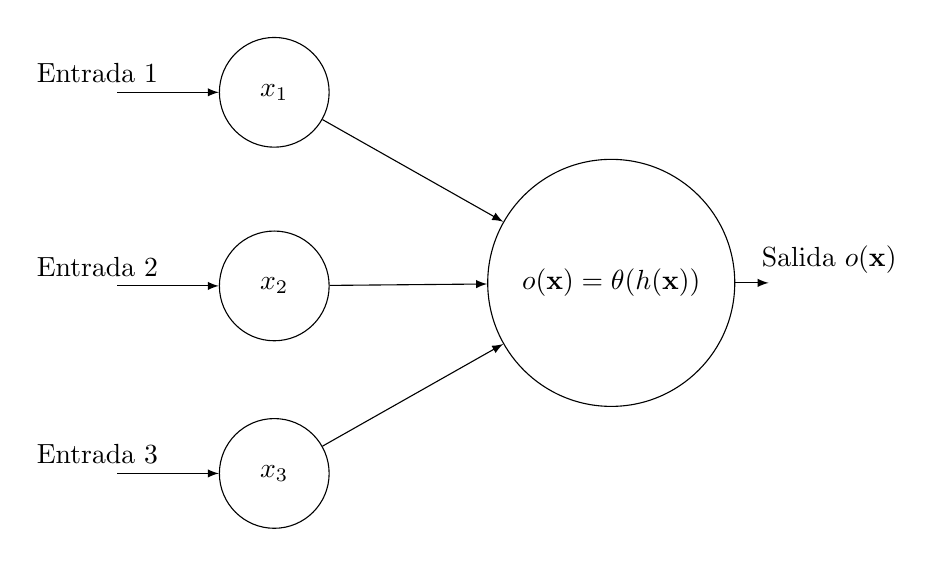
\begin{tikzpicture}[
plain/.style={
  draw=none,
  fill=none,
  },
net/.style={
  matrix of nodes,
  nodes={
    draw,
    circle,
    inner sep=10pt
    },
  nodes in empty cells,
  column sep=2cm,
  row sep=4pt
  },
>=latex
]
\matrix[net] (mat)
{
$x_1$ & |[plain]| \\
$x_2$ &  $ o(\mathbf{x})=\theta(h(\mathbf{x}))$ \\
$x_3$ & |[plain]| \\
};
\foreach \ai [count=\mi ]in {1,2,3}
  \draw[<-] (mat-\ai-1) -- node[above left] {Entrada \mi} +(-2cm,0);
\foreach \ai in {1,2,3}
{\foreach \aii in {2}
  \draw[->] (mat-\ai-1) -- (mat-\aii-2);
}
\draw[->] (mat-2-2) -- node[above right] {Salida $o\mathbf{(x)}$} +(2cm,0);

\end{tikzpicture}


\end{document}